%; whizzy paragraph -pdf xpdf -latex ./whizzypdfptex.sh
%; whizzy-paragraph "^\\\\begin{frame}\\|\\\\emtext"
% latex beamer presentation.
% platex, latex-beamer でコンパイルすることを想定。 

%     Tokyo Debian Meeting resources
%     Copyright (C) 2012 Junichi Uekawa
%     Copyright (C) 2016 Nobuhiro Iwamatsu

%     This program is free software; you can redistribute it and/or modify
%     it under the terms of the GNU General Public License as published by
%     the Free Software Foundation; either version 2 of the License, or
%     (at your option) any later version.

%     This program is distributed in the hope that it will be useful,
%     but WITHOUT ANY WARRANTY; without even the implied warreanty of
%     MERCHANTABILITY or FITNESS FOR A PARTICULAR PURPOSE.  See the
%     GNU General Public License for more details.

%     You should have received a copy of the GNU General Public License
%     along with this program; if not, write to the Free Software
%     Foundation, Inc., 51 Franklin St, Fifth Floor, Boston, MA  02110-1301 USA

\documentclass[cjk,dvipdfmx,12pt]{beamer}
\usetheme{Tokyo}
\usepackage{monthlypresentation}

%  preview (shell-command (concat "evince " (replace-regexp-in-string "tex$" "pdf"(buffer-file-name)) "&")) 
%  presentation (shell-command (concat "xpdf -fullscreen " (replace-regexp-in-string "tex$" "pdf"(buffer-file-name)) "&"))
%  presentation (shell-command (concat "evince " (replace-regexp-in-string "tex$" "pdf"(buffer-file-name)) "&"))

%http://www.naney.org/diki/dk/hyperref.html
%日本語EUC系環境の時
\AtBeginDvi{\special{pdf:tounicode EUC-UCS2}}
%シフトJIS系環境の時
%\AtBeginDvi{\special{pdf:tounicode 90ms-RKSJ-UCS2}}

\newenvironment{commandlinesmall}%
{\VerbatimEnvironment
  \begin{Sbox}\begin{minipage}{1.0\hsize}\begin{fontsize}{8}{8} \begin{BVerbatim}}%
{\end{BVerbatim}\end{fontsize}\end{minipage}\end{Sbox}
  \setlength{\fboxsep}{8pt}
% start on a new paragraph

\vspace{6pt}% skip before
\fcolorbox{dancerdarkblue}{dancerlightblue}{\TheSbox}

\vspace{6pt}% skip after
}
%end of commandlinesmall

\title{Debian Update}
\subtitle{OSC 2021 Onlne/Fall \\東京エリアDebian勉強会(出張版)}
\author{Debian JP Project \\杉本 典充\\ dictoss@debian.or.jp}
\date{2021年10月23日}
\logo{
\includegraphics[width=8cm]{image-assets/openlogo-light.eps}}

\begin{document}

%-------------------

\section{表紙}

\begin{frame}
\titlepage{}
\end{frame}

\section{目次}

\begin{frame}{Agenda}
  \begin{itemize}
  \item Debian とは?
  \item Debian JP Project と Debian 勉強会
  \item Debian 11 (bullseye)
  % \item Debian Updates
  \item 今後のイベント
  \end{itemize}
\end{frame}

%-------------------

\section{Debian とは?}

\begin{frame}
  \begin{center}\Huge{Debian とは?}\end{center}
\end{frame}


\begin{frame}{Debian とは?}

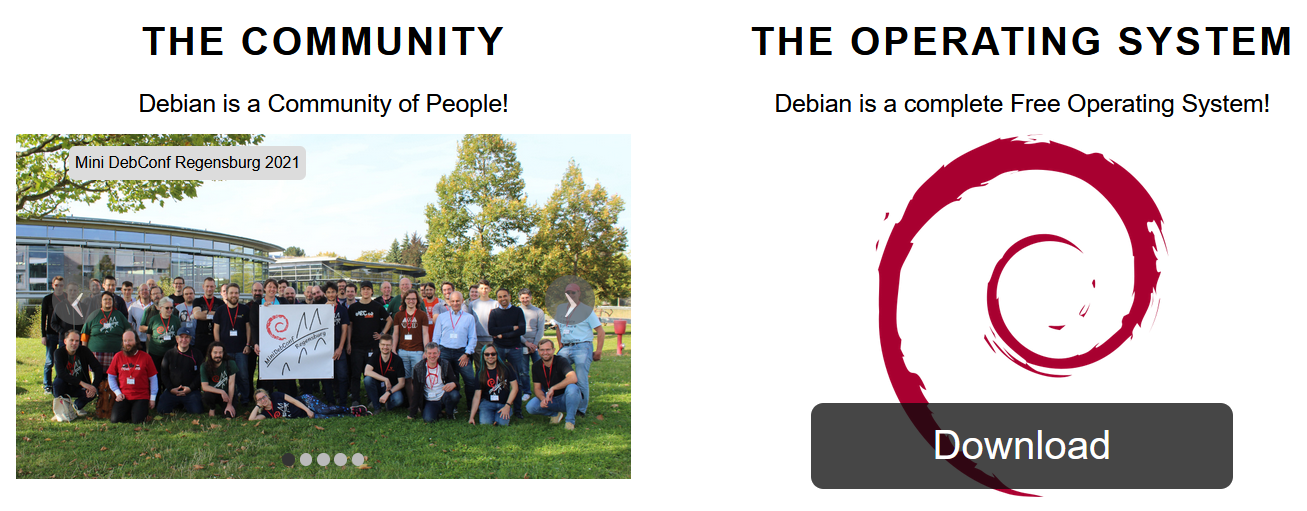
\includegraphics[scale=0.4]{image202110/www-debian-org.png}
%{\small (画像出典:\url{https://www.debian.org/})}

\begin{itemize}
\item \url{https://www.debian.org/}
\item ボランティアで{\color{red}{フリー/オープン}}な{\color{red}{ユニバーサル}}オペレーティングシステム (OS) を開発する「コミュニティ」
\end{itemize}

\end{frame}

\subsection{Debian と OS}

\begin{frame}{Debian というオペレーティングシステム}

\begin{itemize}
\item 様々な用途に使える汎用的な作り
  \begin{itemize}
  \item ノート PC、デスクトップ PC などの普段利用するコンピュータの OS
  \item Linux サーバ
    \begin{itemize}
    \item 例:web サーバのシェア:\url{https://w3techs.com/technologies/details/os-linux/all/all})
    \end{itemize}
  \item 組込デバイスのベース OS (多くの CPU で動作する)
  \end{itemize}
\item 「Debian」ベースな派生OSの源流
  \begin{itemize}
  \item 例:Ubuntu、Kali Linux、Raspberry Pi OS
    % https://debian-handbook.info/browse/en-US/stable/sect.ubuntu.html
    % https://debian-handbook.info/browse/en-US/stable/sect.kali.html
    % https://debian-handbook.info/browse/en-US/stable/sect.raspbian.html
  \item 派生先のディストリビューションと相互に情報交換をして開発している
  \end{itemize}
\end{itemize}

\end{frame}


\begin{frame}{Debian というオペレーティングシステム}
\
  \begin{itemize}
  \item 2021 年 10 月の時点で、最新版は {\color{red}{Debian 11.1}} (コードネーム: bullseye)
    \begin{itemize}
    % https://www.debian.org/releases/bullseye/amd64/release-notes/ch-whats-new.ja.html
    \item パッケージ数は {\color{red}{約59,551}} 以上を提供
    \item 公式にサポートする CPU アーキテクチャは {\color{red}{9}}
    \end{itemize}
  \item コードネームはトイ・ストーリーのキャラクター名を採用
  \item 次のメジャーリリース は Debian 12 (コードネーム: {\color{red}{}}bookworm)
%    \begin{itemize}
%    \item 2023 年中頃にリリースすると思われる
%    \end{itemize}
\end{itemize}

\end{frame}


\begin{frame}{Debian というオペレーティングシステム}

リリースサイクル

\begin{itemize}
\item メジャーリリース:おおよそ 2 年ごと
  \begin{itemize}
  \item Debian は time-based freeze を採用
    % https://www.debian.org/News/2009/20090729
  \end{itemize}
\item 標準サポート期間:3年
  % https://www.debian.org/releases/
\item LTS(Long Term Support):標準サポート期間終了後から 2 年
  % https://wiki.debian.org/LTS
  \begin{itemize}
  \item サポートするアーキテクチャが amd64、i386、arm 系に絞られる
  \item 全パッケージをサポートするわけではなく、主要なパッケージに絞ってサポート
  %\item スポンサーとして資金援助するとメンテナンスするパッケージの希望を出せる
  \end{itemize}
\end{itemize}

\end{frame}


\subsection{Debian と コミュニティ}

\begin{frame}{Debian というコミュニティ}

Debian への参加者は世界中にいます

\begin{itemize}
\item 公式の Debian 開発者(Debian Developer)は、60 ヶ国以上に約 1,100 名
  % https://www.debian.org/intro/why_debian
  % https://db.debian.org/
\item パッケージメンテナや翻訳などの貢献者も入れるともっと多くの人たちが参加
\end{itemize}
  
\end{frame}


\begin{frame}{Debian というコミュニティ}

\begin{itemize}
\item Debian 社会契約
  \begin{itemize}
  \item Debian 開発者 たちが目指すフリーソフトウェアコミュニティの在り方
  \end{itemize}
\item Debian フリーソフトウェアガイドライン(DFSG)
  \begin{itemize}
  \item Debian 社会契約の一部
  \item Debian が考えるフリーソフトウェアの定義
  \item オープンソースの定義のひな形にもなっている
  \end{itemize}
\item Debian Policy
  \begin{itemize}
  \item \url{https://www.debian.org/doc/debian-policy/}
  \item Debian パッケージの区分、内容、ルール、ファイル配置の方針などの技術的な定義
  \end{itemize}
\end{itemize}

\end{frame}


\begin{frame}{Debian というコミュニティ}

Debian はボランティアのみで開発しています

\begin{table}[htb]
  \begin{tabular}{|c|c|c|}
    \hline
    ディストリ & 企業 & ボランティア \\ \hline
    Fedora & RedHat支援あり & あり  \\ \hline
    RHEL & RedHat & なし  \\ \hline
    CentOS & RedHat支援あり & あり \\ \hline
    \color{red}{Debian}  & \color{red}{なし} & \color{red}{あり} \\ \hline
    Ubuntu  & Canonical & あり \\ \hline
    openSUSE & SUSE支援あり & あり \\ \hline
    SLES & SUSE & なし \\ \hline
  \end{tabular}
\end{table}

\end{frame}


\begin{frame}{DebConf}%[containsverbatim]
  
\begin{itemize}
\item 年に一回、Debian 開発者が集まって開催するカンファレンス
\item 通常はオフラインで集まるが、COVID-19 の影響で 2020 年と 2021 年はオンラインで開催
  \begin{itemize}
  \item 2019/07/21 - 07/28: Debconf19: CURITIBA - BRAZIL
  \item 2020/08/23 - 08/29: Debconf20: Online
  \item 2021/08/24 - 08/28: Debconf21: Online
    \begin{itemize}
    \item \url{https://debconf21.debconf.org/}
    \item 発表のビデオがありますのでぜひご覧ください
    \end{itemize}
  \end{itemize}
\end{itemize}

%\begin{center}
  %\includegraphics[scale=0.2]{image202110/dc21group-photo-25percent.png}
  %% https://wiki.debian.org/DebConf/21/GroupPhoto?action=AttachFile&do=get&target=dc21group-photo-25percent.png
%\end{center}

\end{frame}

\subsection{まとめ}

\begin{frame}{Debian とは?}
  
まとめると「Debian」とは

\begin{itemize}
  \item フリー/オープンなオペレーティングシステム (OS) を作成しようとする人たちが集まるボランティアベースのプロジェクト
  \item 自分たちの考えるフリーという言葉に関する定義、開発目的、パッケージングポリシーを厳格に決めている
  \item 世界中に 1100 人以上の開発者がおり、他のディストリビューションのベースとして採用されている
  \item 約 2 年毎にリリースが行われ、多くのパッケージとアーキテクチャをサポートしている
  \item 上記のような特徴から様々なところで利用されている Linux ディストリビューション
\end{itemize}

\end{frame}

%------------------


\section{Debian JP Project と Debian勉強会}


\begin{frame}
  \begin{center}\Huge{Debian JP Project\\と\\Debian勉強会}\end{center}
\end{frame}

\subsection{Debian JP Projectとは}
  
\begin{frame}{Debian JP Project とは?}

\begin{itemize}
  \item \url{https://www.debian.or.jp/}
  \item 日本において Debian を普及させることを目的とした任意団体
  \item 活動内容
  \begin{itemize}
    \item Debian の日本語による情報発信
    \item ユーザとの情報交換
    \item Debian 開発者やパッケージメンテナの育成など
  \end{itemize}
\end{itemize}

\end{frame}


\subsection{Debian勉強会}


\begin{frame}{Debian勉強会}

\begin{itemize}
 \item 2005 年 1月開始
 \item Debian 開発者 上川さんが発起人
 \item 東京と関西で月に一回コンスタントに開催しているDebian 開発者、Debian ユーザによる勉強会
   \begin{itemize}
   \item 東京エリアDebian勉強会
     \begin{itemize}
     \item \url{https://tokyodebian-team.pages.debian.net/}
     \end{itemize}
   \item 関西Debian勉強会
     \begin{itemize}
     \item \url{https://wiki.debian.org/KansaiDebian}
     \end{itemize}
   \end{itemize}
\end{itemize}

\end{frame}


\begin{frame}{Debian勉強会:解決したい内容}

\begin{itemize}
 \item 問題
   \begin{itemize}
   \item ML と IRC で情報交換していた
   \item face-to-face で会う場所がない
   \item まとまったドキュメントが出てこない
   \end{itemize}
 \item Debian 勉強会の提案
   \begin{itemize}
   \item 定期的に集まる
   \item 資料を作成して公開(GPL-2+) \\
	 {\small \url{https://salsa.debian.org/tokyodebian-team/monthly-report}}
   \end{itemize}
\end{itemize}

\end{frame}


\subsection{最近の勉強会}


\begin{frame}{Debian勉強会:最近の勉強会}
  
\begin{itemize}
\item 勉強会の内容
  \begin{itemize}
  \item Debian 界隈やパッケージング関連の話題など専門の人に話を聞く
  \item Debianで気になった事柄を調べてレポートする
  \end{itemize}
\item 前回の内容(東京 9月):
  \begin{itemize}
  \item 場所: オンライン
  \item DebConf 21 のイベント共有会
  \end{itemize}
\item 各地のイベントでDebian普及活動
  %\begin{itemize}
  %\item OSC2019北海道、OSC2019京都、OSC2019東京
  %\item 関西オープンフォーラム
  %\end{itemize}
\end{itemize}

\end{frame}

%-----------------------

\section{Debian 11 bullseye}

\begin{frame}
  \begin{center}\Huge{Debian 11 bullseye\\リリースおめでとう!}\end{center}
\end{frame}

\subsection{リリース情報}

\begin{frame}{Debian 11 bullseye}% [containsverbatim]

Debian 11 (コードネーム:bullseye)

\begin{itemize}
\item 2021 年 8 月 14 日にリリース
\item 最新版は Debian 11.1 (2021 年 10 月 9 日 リリース)
\item リリースノート
  \begin{itemize}
    \item \url{https://www.debian.org/releases/bullseye/releasenotes}
  \end{itemize}
\item インストールガイド
  \begin{itemize}
    \item \url{https://www.debian.org/releases/bullseye/installmanual}
  \end{itemize}  
\end{itemize}

%\begin{center}
  %\includegraphics[width=0.6\hsize]{image201902/bullseye.jpg}
  % https://pixar.fandom.com/wiki/Bullseye
%\end{center}

\end{frame}


\subsection{CPUアーキテクチャ}

\begin{frame}{Debian 11 bullseye}% [containsverbatim]

利用できる CPU アーキテクチャは 9 つ

\begin{itemize}
\item amd64、i386
\item arm64、armhf、armel
\item mips64el、mipsel
\item ppc64el
\item s390x
\end{itemize}

前回リリース Debian 10 buster から廃止
\begin{itemize}
\item (big endian の) mips
\end{itemize}

\end{frame}


\subsection{提供するソフトウェア}

\begin{frame}{Debian 11 bullseye}% [containsverbatim]

提供するソフトウェア(1)

\begin{multicols}{2}

  \begin{table}[htb]
    \begin{tabular}{|c|c|}
      \hline
      Linux kernel & 5.10 \\ \hline
      GNOME & 3.38 \\ \hline
      KDE Plasma & 5.20 \\ \hline
      LXDE & 11 \\ \hline
      LXQt & 0.16 \\ \hline
      MATE & 1.24 \\ \hline
      Xfce & 4.16 \\ \hline
      Cinnamon & 4.8.6 \\ \hline
      Chromium & 90.0 \\ \hline
      OpenSSH & 8.4p1 \\ \hline
      OpenSSL & 1.1.1k \\ \hline
      GnuPG & \begin{tabular}{c} 2.2.27 \\ 1.4.23\end{tabular} \\ \hline
    \end{tabular}
  \end{table}

  \newpage

  \begin{table}[htb]
    \begin{tabular}{|c|c|}
      \hline
      Firefox ESR & 78 \\ \hline
      Thunderbird & 78 \\ \hline
      LibreOffice & 7.0 \\ \hline
      GIMP & 2.10.22 \\ \hline
      Inkscape & 1.0.2 \\ \hline
      MariaDB & 10.5 \\ \hline
      PostgreSQL & 13 \\ \hline
      sqlite & \begin{tabular}{c} 3.34.1 \\ 2.8.17 \end{tabular} \\ \hline
      Emacs & 27.1 \\ \hline
      Vim & 8.2 \\ \hline
    \end{tabular}
  \end{table}

\end{multicols}

\end{frame}


\begin{frame}{Debian 11 bullseye}% [containsverbatim]

提供するソフトウェア(2)

\begin{multicols}{2}

  \begin{table}[htb]
    \begin{tabular}{|c|c|}
      \hline
      Perl & 5.32.1 \\ \hline
      PHP & 7.4 \\ \hline
      Python & \begin{tabular}{c} 3.9.1 \\ 2.7.18 \end{tabular} \\ \hline
      Ruby & 2.7.4 \\ \hline
      OpenJDK & \begin{tabular}{c} 11 \\ 17 \end{tabular} \\ \hline
      Go & 1.15 \\ \hline
      Rustc & 1.48 \\ \hline
      GCC & 10.3 \\ \hline
      LLVM & \begin{tabular}{c} 11.0.1 \\ 9.0.1 \end{tabular} \\ \hline
      binutils & 2.35.2 \\ \hline
      glibc & 2.31 \\ \hline
    \end{tabular}
  \end{table}

\end{multicols}

\end{frame}

%-----------------------

\subsection{新機能}

\begin{frame}
  \begin{center}\Huge{Debian 11 bullseye の\\新機能}\end{center}
\end{frame}


\begin{frame}{新機能 (1)}

システム全体の新機能
  
\begin{itemize}
\item コントロールグループ v2 (cgroupv2)
  \begin{itemize}
  \item bullseye における systemd はデフォルトで cgroupv2 を利用
  \end{itemize}
\item systemd の永続的なジャーナル機能はデフォルトで有効
  \begin{itemize}
  \item ファイルを /var/log/journal/ 配下に保存するよう変更
  \item ファイルは adm グループも読み取りできるため注意
  \end{itemize}
\item カーネルによる exFAT サポート
  \begin{itemize}
  \item Debian 10 buster で exFAT を利用するために必要であった exfat-fuse パッケージが不要になった
  \end{itemize}
\item 新しい汎用的な open コマンド
  \begin{itemize}
  \item ファイルの拡張子ごとに適切なコマンドでファイルを開けるようになった
  \end{itemize}  
\end{itemize}
  
\end{frame}


\begin{frame}{新機能 (2)}

アプリケーションの新機能
  
\begin{itemize}
\item ドライバレスでのスキャンと印刷
  \begin{itemize}
  \item 印刷では IPP-over-USB プロトコルを扱える新しい ipp-usb パッケージを提供
  \item スキャナでは公式の SANE ドライバレスバックエンドである libsane1 を提供 
  \end{itemize}
\item 新しい Fcitx 5 インプットメソッド
  \begin{itemize}
  \item Fcitx 5 は中国語、日本語、韓国語やその他の多くの言語のためのインプットメソッド
  \item Fcitx 5 では Wayland をサポートし、より優れたアドオンサポートを提供
  \end{itemize}
\end{itemize}
  
\end{frame}


\begin{frame}{新機能 (3)}

その他の新機能
  
\begin{itemize}
\item Debian Med チームによる貢献の反映
  \begin{itemize}
  \item 疫学方面で利用されるツールのソフトウェアをパッケージ化
  \item 生命科学と医学の分野における新しいパッケージを追加
  \item 既存のパッケージに対する継続的インテグレーションのサポート強化
  \end{itemize}
\item man ページの翻訳の改善
  \begin{itemize}
  \item bullseye リリースが存続する期間中は翻訳の改善を backports アーカイブ経由で提供予定
  \end{itemize}
\item 代替 init システムのサポート改善
  \begin{itemize}
  \item デフォルトは systemd
  \item 代替 init システム (System-V 形式の init や OpenRC など) をサポート
  \end{itemize}
\end{itemize}

\end{frame}


\subsection{アップグレード時の注意}

\begin{frame}[containsverbatim]{アップグレードする場合の注意}

apt のセキュリティアーカイブの構成 (=URL) が変更されたため、手動で書き換えをお願いします

\begin{commandlinesmall}
# vi /etc/apt/sources.list
  
# debian 10 buster
deb http://security.debian.org/debian-security buster/updates main contrib

↓

# debian 11 bullseye
deb https://deb.debian.org/debian-security bullseye-security main contrib
\end{commandlinesmall}

アップグレードの最中に 新たに ssh 接続ができない時間が長くなっているため、ssh 接続してアップグレードする場合は以下の手順がおすすめ

\begin{itemize}
\item /etc/apt/sources.list を書き換える
\item apt-get update を実行する
\item apt-get install openssh-server を実行する
\item apt-get upgrade、apt-get dist-upgrade を実行する
\end{itemize}

\end{frame}


\begin{frame}{動作の変更や制約 (1)}% [containsverbatim]

\begin{itemize}
\item Intel 社製 GPU のデフォルトドライバーが新しい VA-API に変更
\item XFS ファイルシステムは barrier/nobarrier オプションをサポートしない
\item パスワードのハッシュ化に yescrypt をデフォルトで利用するよう変更
\item NSS NIS および NIS+ 利用に新しいパッケージが必要
\item unbound での分割された設定ファイルの扱い
\item 非推奨になる rsync のパラメータ
\item Vim のアドオンの取り扱いの変更
\item OpenStack と cgroups v1 について
\item OpenStack API ポリシーのファイルについて
\item アップグレード中の sendmail にダウンタイムがある
\item fuse から fuse3 へアップグレード処理で fuse パッケージを削除する
\end{itemize}

\end{frame}


\begin{frame}{動作の変更や制約 (2)}% [containsverbatim]

\begin{itemize}
\item GnuPG オプションファイルの変更
\item Linux がユーザー名前空間をデフォルトで有効にする
\item Linux が bpf() の非特権呼び出しをデフォルトで無効
\item bullseye に redmine がない
\item bullseye の Exim 4.94 は実質メジャーアップデート
\item SCSI デバイスの検出順が決定的ではなくなった
\item rdiff-backup は サーバーとクライアントを同時にアップグレードする必要あり
\item Intel CPU のマイクロコードでの問題
\item libgc1c2 パッケージ関連のアップグレードは 2 回実行が必要
\item fail2ban が bsd-mailx の mail コマンドを使ったメール送信ができない
\end{itemize}

\end{frame}


\begin{frame}{非推奨になった事項 (1)}% [containsverbatim]

linuxカーネル、ブートローダー関連
  
\begin{itemize}
\item Linuxカーネルは isdn4linux (i4l) のサポートを提供しない
\item aufs-dkms は bullseye から削除
  \begin{itemize}
  \item overlayfs への移行を推奨
  \end{itemize}    
\item lilo は bullseye から削除
  \begin{itemize}
  \item grub2 を利用してください
  \end{itemize}    
\item armel、armhf利用者向け
  \begin{itemize}
  \item 以下ハードウェア向けの kernel をビルドできなくなったため、Debian 11 bullseye ではサポートされない
    \begin{itemize}
    \item QNAP Turbo Station (TS-xxx)
    \item HP Media Vault mv2120 
    \end{itemize}
  \end{itemize}  
\end{itemize}

\end{frame}


\begin{frame}{非推奨になった事項 (2)}% [containsverbatim]

アプリケーション関連
  
\begin{itemize}
\item ネットワーク接続マネージャーである wicd は、アップグレード後には利用できない
\item libappindicator ライブラリは提供されない
  \begin{itemize}
  \item fork である libayatana-appindicator を提供するよう切り替え
  \end{itemize}  
\item bullseye では chef を提供されない
  \begin{itemize}
  \item 最もよい移行先は Chef Inc が提供するパッケージへの切り替え
  \end{itemize}
\item (mailman2 の) mailman パッケージが廃止され、 mailman3 のみ提供
\item python2.7 パッケージは提供するが upstream が EoL のため python3 への移行を推奨
  \begin{itemize}
  \item bullseye では python2.7 関連のライブラリパッケージの大部分を削除済み
  \item Debian 12 で python2.7 の提供をやめるかどうかは議論中
  \end{itemize}
\end{itemize}

\end{frame}


\subsection{バグレポート}

\begin{frame}{バグレポートをお願いします}% [containsverbatim]
  \begin{itemize}
  \item 何かおかしい動作や不具合を見つけた場合はバグレポートをお願いします
  \item バグレポートの例 \url{https://bugs.debian.org/cgi-bin/bugreport.cgi?bug=903529}
  \item バグレポートの仕方(レポートは英語で送る必要あり)
    \begin{itemize}
    \item \url{https://www.debian.org/Bugs/Reporting.ja.html}
    \end{itemize}
  \item バグレポートの前にちょっと相談してみたい方は、日本語の Debian JP メーリングリストや、SNSで相談してみてください
    \begin{itemize}
    \item \url{https://www.debian.or.jp/community/ml/openml.html}
    \item Twitter: @debian\_jp
    \end{itemize}
  \end{itemize}
\end{frame}

%-----------------------

%\section{Debian Updates}

% 半年間の以下MLから抜粋して紹介する
%  debian-announce@lists.debian.org
%  debian-devel-announce@lists.debian.org

%\begin{frame}
%  \begin{center}\Huge{Debian Updates}\end{center}
%\end{frame}


%\subsection{released timeline}

%\begin{frame}{Debian Updates}% [containsverbatim]

%\begin{itemize}
%\item 2021/02/06:  Updated Debian 10.8  released
%\item 2021/03/27:  Updated Debian 10.9  released
%\item 2021/06/19:  Updated Debian 10.10 released
%\item 2021/08/14:  Debian 11 released
%\item 2021/10/09:  Updated Debian 10.11 released
%\item 2021/10/09:  Updated Debian 11.1  released
%\end{itemize}

%\end{frame}


%\subsection{Bits from the DPL}

%\begin{frame}{Debian Updates}% [containsverbatim]

%Bits from the DPL

%\begin{itemize}
%\item 月に一度の Debian Project Leader である jcc さんのプロジェクトの進捗を報告
%\item 時間のない方でもこれを読んでおけば Debian Project の大まかな動きがわかる
%\end{itemize}

%\small{
%\begin{itemize}

%\item 2021/08/30 \url{https://lists.debian.org/debian-devel-announce/2021/08/msg00005.html}

%\end{itemize}
%}

%\end{frame}


%-----------------------

\section{日本語によるDebianの情報}

\begin{frame}\begin{center}\Huge{日本語によるDebianの情報}\end{center}\end{frame}

\begin{frame}{日本語によるDebianの情報}
\begin{itemize}
  \item Debian JP Project \\
      \url{https://www.debian.or.jp}
  \item 東京エリアDebian勉強会\\
      \url{https://tokyodebian-team.pages.debian.net/}
  \item 関西Debian勉強会 \\
      \url{https://wiki.debian.org/KansaiDebianMeeting}
  \item Twitter \\
      \url{@debian_jp}
  \item 雑誌 Software Design 技術評論社発行 \\
    「Debian Hot Topics」(隔月連載)
\end{itemize}
\end{frame}

%----------------

\section{今後のイベント}

\begin{frame}\begin{center}\Huge{今後のイベント}\end{center}\end{frame}


\begin{frame}{今後のイベント}

\begin{itemize}
\item 11/21(日) 東京エリア・関西合同 Debian 勉強会(オンライン開催)
  \begin{itemize}
  \item \url{https://tokyodebian-team.pages.debian.net/2021-11.html}
  \item OSS Gate オンボーディング実施報告
  \end{itemize}
\end{itemize}

\end{frame}

%----------------

\end{document}

;;; Local Variables: ***
;;; outline-regexp: "\\([ 	]*\\\\\\(documentstyle\\|documentclass\\|emtext\\|section\\|begin{frame}\\)\\*?[ 	]*[[{]\\|[]+\\)" ***
;;; End: ***
